\begin{figure}[h!]
	\begin{subfigure}{0.5\textwidth}
		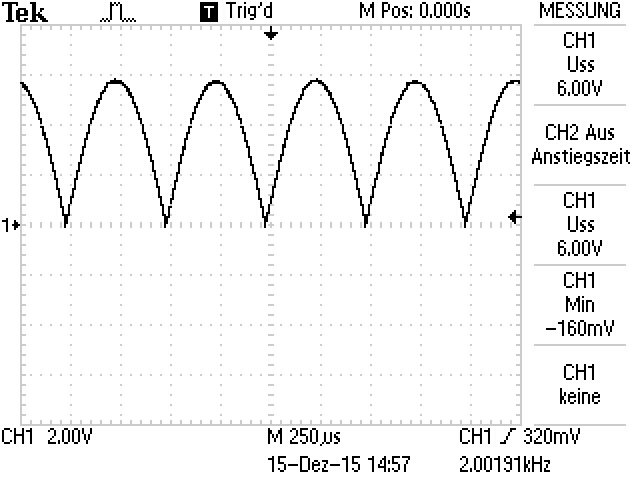
\includegraphics[width = \textwidth]{Oszilloskop-Bilder/ohne_345.JPG}
		\caption{ohne Rauschen}
	\end{subfigure}
	\begin{subfigure}{0.5\textwidth}
		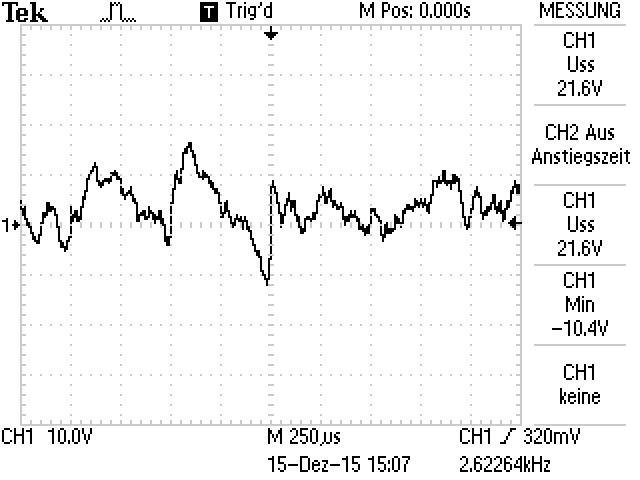
\includegraphics[width = \textwidth]{Oszilloskop-Bilder/mit_345.JPG}
		\caption{mit Rauschen}
	\end{subfigure}
	\caption{Spannungsmischung bei einer Phasendifferenz von $\Delta\phi = \SI{0}{\degree}$}
	\label{Verschiebung_0}
\end{figure}

\begin{figure}[h!]
	\begin{subfigure}{0.5\textwidth}
		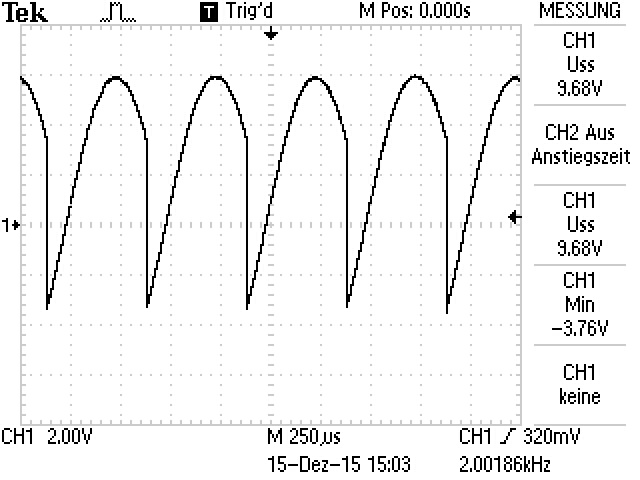
\includegraphics[width = \textwidth]{Oszilloskop-Bilder/ohne_30.JPG}
		\caption{ohne Rauschen}
	\end{subfigure}
	\begin{subfigure}{0.5\textwidth}
		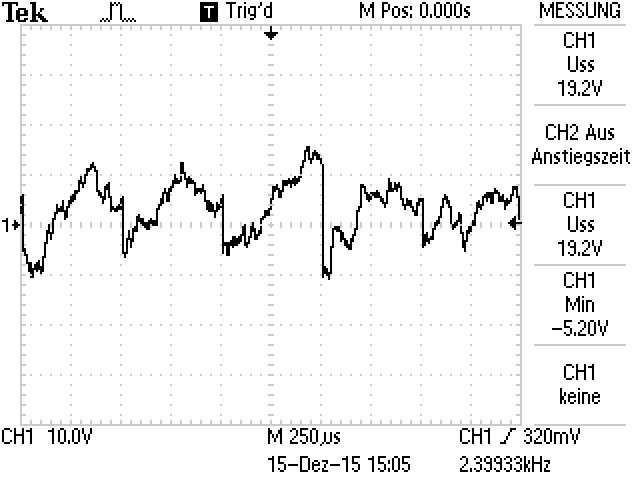
\includegraphics[width = \textwidth]{Oszilloskop-Bilder/mit_30.JPG}
		\caption{mit Rauschen}
	\end{subfigure}
\caption{Spannungsmischung bei einer Phasendifferenz von $\Delta\phi = \SI{45}{\degree}$}
\end{figure}

\begin{figure}
	\begin{subfigure}{0.5\textwidth}
		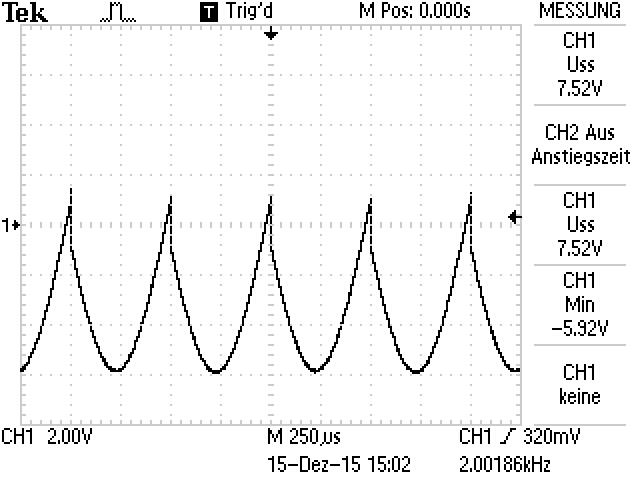
\includegraphics[width = \textwidth]{Oszilloskop-Bilder/ohne_150.JPG}
		\caption{ohne Rauschen}
	\end{subfigure}
	\begin{subfigure}{0.5\textwidth}
		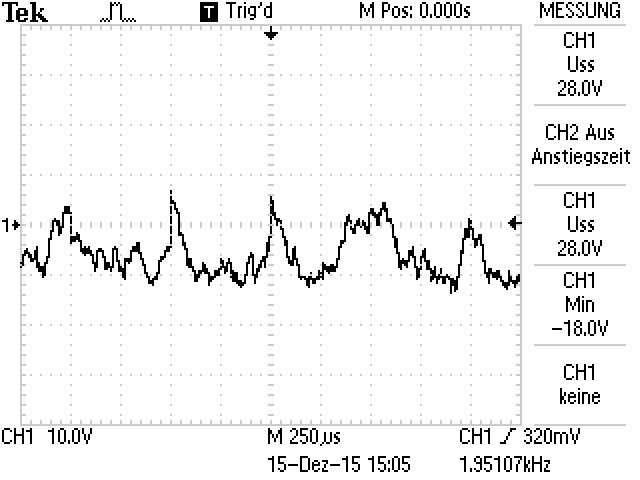
\includegraphics[width = \textwidth]{Oszilloskop-Bilder/mit_150.JPG}
		\caption{mit Rauschen}
	\end{subfigure}
\caption{Spannungsmischung bei einer Phasendifferenz von $\Delta\phi = \SI{165}{\degree}$}
\end{figure}

\begin{figure}
	\begin{subfigure}{0.5\textwidth}
		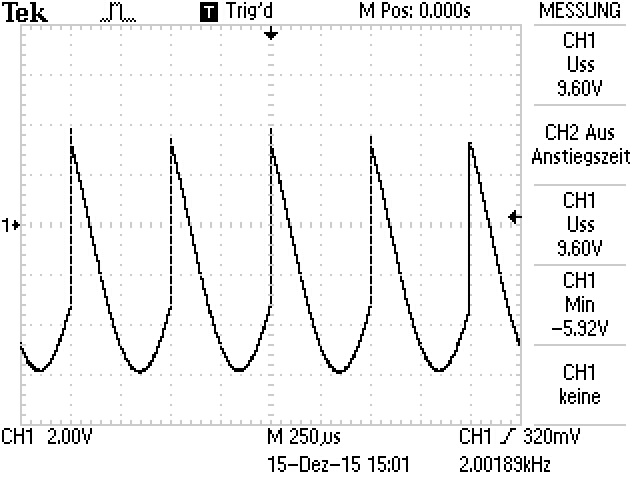
\includegraphics[width = \textwidth]{Oszilloskop-Bilder/ohne_210.JPG}
		\caption{ohne Rauschen}
	\end{subfigure}
	\begin{subfigure}{0.5\textwidth}
		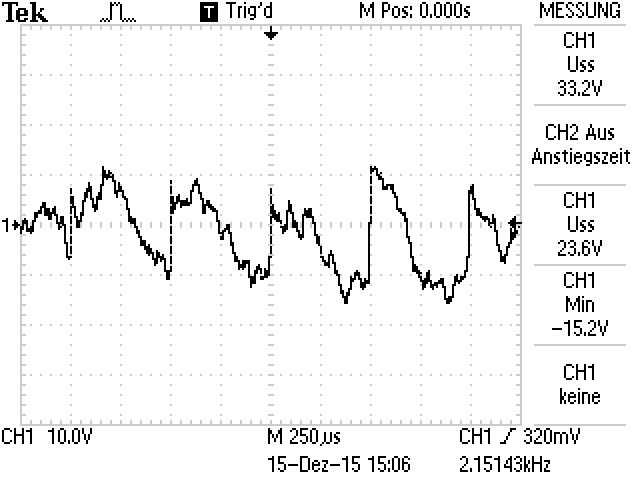
\includegraphics[width = \textwidth]{Oszilloskop-Bilder/mit_210.JPG}
		\caption{mit Rauschen}
	\end{subfigure}
\caption{Spannungsmischung bei einer Phasendifferenz von $\Delta\phi = \SI{225}{\degree}$}
\end{figure}

\begin{figure}
	\begin{subfigure}{0.5\textwidth}
		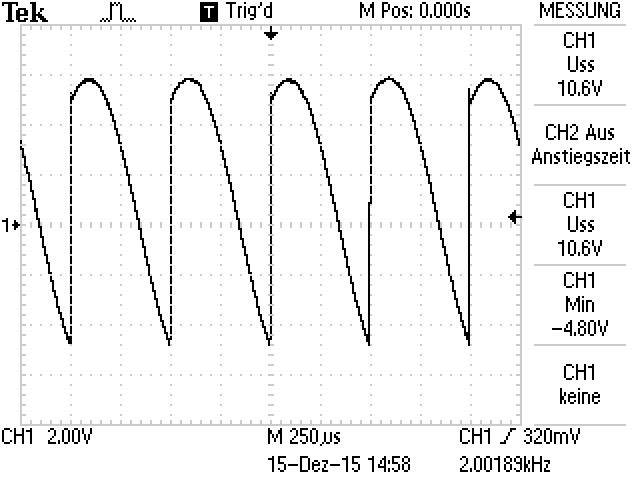
\includegraphics[width = \textwidth]{Oszilloskop-Bilder/ohne_300.JPG}
		\caption{ohne Rauschen}
	\end{subfigure}
	\begin{subfigure}{0.5\textwidth}
		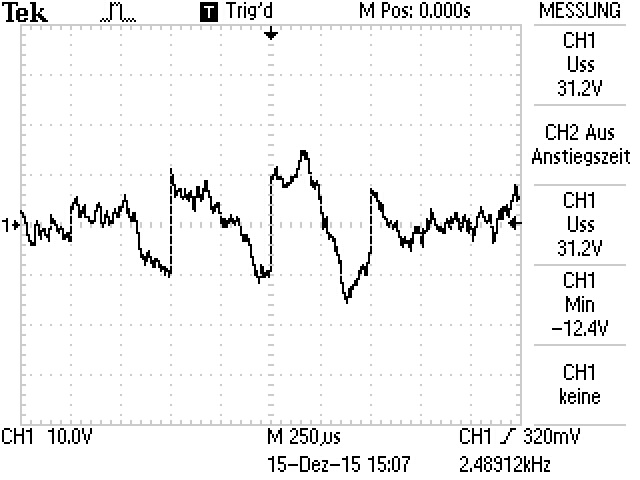
\includegraphics[width = \textwidth]{Oszilloskop-Bilder/mit_300.JPG}
		\caption{mit Rauschen}
	\end{subfigure}
\caption{Spannungsmischung bei einer Phasendifferenz von $\Delta\phi = \SI{315}{\degree}$}
\label{Verschiebung_315}
\end{figure}